\documentclass{cmspaper}
\usepackage{multirow}
\begin{document}

%==============================================================================
% title page for few authors

\begin{titlepage}

% select one of the following and type in the proper number:
   \cmsnote{2009/XXX}
%  \internalnote{2005/000}
%  \conferencereport{2005/000}
   \date{1 Aug 2009}

  \title{Persistent storage of non event data in the CMS databases}

  \begin{Authlist}
    M.De Gruttola \Aref{a}, P.Paolucci 
        \Instfoot{cern}{CERN, Geneva, Switzerland}
        \Instfoot{ieph}{INFN Sezione di Napoli, Naples, Italy}
    S.Di Guida, D.Futyan, G. Govi, V.Innocente,  F.Glege, P.Picca, A.Pierro, D.Schlatter, Z.Xie
          \Instfoot{cern}{CERN, Geneva, Switzerland}
 %  D.~Author, E.~Author\Aref{b}, F.~Author
  %     \Instfoot{ieph}{Institute of Experimental Physics, Hepcity, Wonderland}
  \end{Authlist}

% if needed, use the following:
%\collaboration{Flying Saucers Investigation Group}
%\collaboration{CMS collaboration}

  \Anotfoot{a}{Also with {\it{Universit\`a  degli studi di Napoli ``Federico II'', Naples, Italy}}}
%  \Anotfoot{b}{Now at the Moon}

  \begin{abstract}

  \end{abstract} 
In the CMS experiment the non event data needed to set up the detector, or being  produced by it, and needed to calibrate the physical responses of the detector itself are stored in ORACLE databases. The large amount of data to be stored, the number of clients involved and the performance requirements make the database system an essential service for the experiment to run. This note describes the CMS condition database architecture, the dataflow and PopCon, the tool built to populate the offline databases. The first results obtained during the 2008 and 2009 cosmic data taking are presented.
% if needed, use the following:
%\conference{Presented at {\it Physics Rumours}, Coconut Island, April 1, 2005}
%\submitted{Submitted to {\it Physics Rumours}}
%\note{Preliminary version}
  
\end{titlepage}

\setcounter{page}{2}%JPP

\tableofcontents

\section{Introduction}

Databases have become a vital part of the LHC experiments. 
The large amount of data needed to set up the detector (tens of GBytes) and produced by (few terabytes per year) it makes the DB system an indispensable service for CMS to run. 
During the construction phase many databases, based on different technologies and software, were developed by the subproject to store all the detector and equipment data. 
In the 2004, the CMS collaboration, decided to start a common and central project, called CMS DB project, in order to converge towards an unique database technology and a set of central software tools supported by the experiment for whole data tacking. 

The current layout of the database model and dataflow was developed after two workshops and one review and working hardly with the CMS subsystems.
 
The two most important requirements identified by CMS are:
\begin{itemize}
\item	CMS has to be able to operate without network connection between P5 and the outside world (CERN network included). Therefore CMS must possess an independent database structure based at P5.
\item	Offline condition data work-flow has to follow the multi-tier dislocation structure as the event data one. 
\end{itemize}
The DB project group, with the help of IT and in collaboration with all the CMS subprojects, designed a system based on 3 different databases based on the ORACLE technology. 
\begin{itemize}
\item	 Online Master Database System ({\bf{OMDS}}) is the online master database placed at P5 on the CMS online network. It stores the configuration of the detector and the non event data (condition data) produced by the subsystems (slow control, electronics, DAQ and trigger data). It is a purely relational database.

\item  Offline Reconstruction Condition DB ONline subset ({\bf{ORCON}}) stores all the condition data needed online by the HLT. It also contains part of the online data stored in OMDS and needed offline for data quality indicator and for more detailed offline analysis.
The data in it are written using the POOL-ORA\cite{POOLORA} technology and are retrieved by the HLT programs as {\texttt{C++}} objects for the offline software.  

\item  Offline Reconstruction Condition DB Offline subset ({\bf{ORCOFF}}) is the master offline database placed at IT and it contains a copy of ORCON made through the ORACLE streaming.
Data in it are retrieved by the reconstruction algorithms as \texttt{C++} objects for the offline software. 
\end{itemize}


%A sketch of the CMS condition data work-flow is shown in figure~\ref{fig:ConditionDataflow}. 

%\begin{figure}[hbtp]
%   \begin{center}
%    \resizebox{0.8\textwidth}{!}{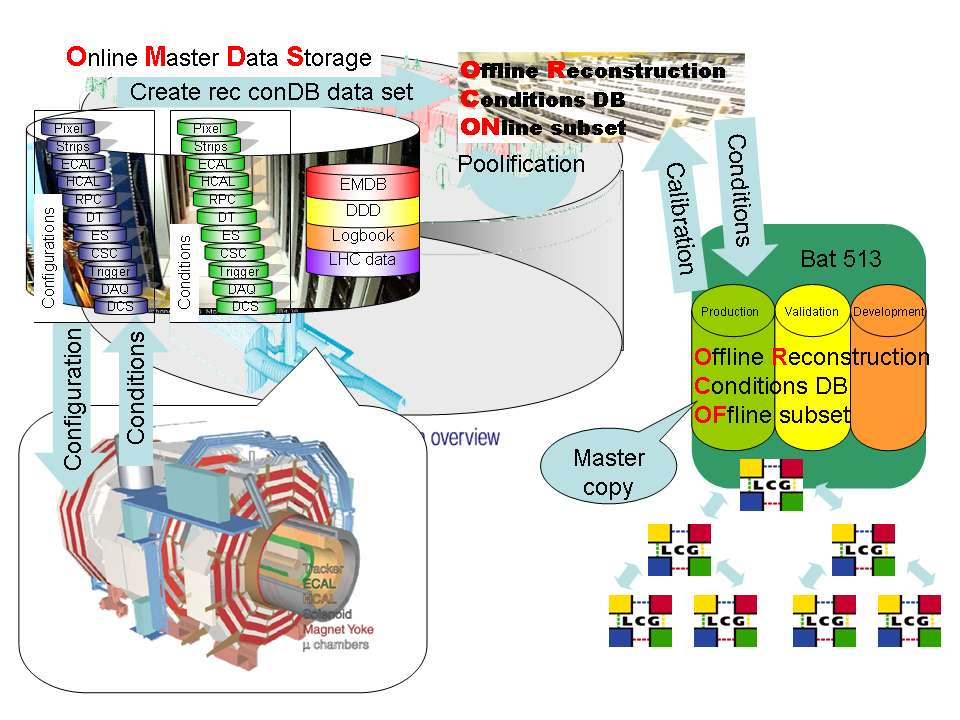
\includegraphics{figure/db-model.jpg}}
%\caption{Data-flow of non event data in CMS.}
%    \label{fig:ConditionDataflow}
%  \end{center}
%\end{figure}


\section{Online Master database}
In CMS the non event data needed to set up the detector or being produced by the detector will be stored in OMDS, which is a Relational ORACLE database.
The data has been classified primarily according to its needs for meta data (data to describe the data) as follows:

{\bf {Construction data}} During production of the detector data is gathered about the production process and the produced items. Some of the construction data also belongs into the data classes described here after and will
therefore be moved to the common data storage at the end of construction. The CMS detectors agreed to
keep their construction data available for the lifetime of the experiment to be able to trace back production
errors. The construction data and it�s storage will not be described in this document.


{\bf {Equipment management data}} Detector items should be tracked to log their history of placements and repairs.
The classification of CERN as INB (Installation Nucleaire de Base) requires in addition, to keep a continuous
trace of the location of irradiated items. Equipment management data contains therefore this location history
of all items being installed at the experiment. It contains detector parts as well as off detector electronics.
The required meta data is the interval of validity (IOV).


{\bf{Configuration data}} The data needed to bring the detector in any running mode is classified as configuration
data. This comprises voltage settings of power supplies as well as programmable parameters for front end
electronics. Configuration data requires version and tag as meta data.

{\bf{Conditions data}} There are two main uses of conditions data: In the online system conditions data is used for
post mortem analysis of detector errors. In the offline the conditions are needed for event reconstruction as
well as data quality indicator. The conditions needed offline are a sub set of the online conditions. The conditions meta data are interval of validity, version and tag. 

The general data flow can be described as follows (see figure \ref{fig:CondDBArchitecture}): every subproject calculates and measures in advance all the parameters needed to setup his hardware devices, mainly related to the detector, DAQ and trigger. Different hardware setup can be stored at same time in the configuration database but only one will be loaded before the run starts. While running, the detector produces many kind of conditions, to be stored in OMDS, from the slow control (PVSS \cite{PVSS}) and from other tools like DAQ (XDAQ), Run Control and data quality monitor (DQM). 
Part of OMDS data, needed to the HLT and to the offline, will be transfer to ORCON (the O2O procedure is called PopCon ) and then streamed to ORCOFF (more details in the section \ref{OffDB}). 
When a new set of calibrations, calculated offline using event data and the related condition data, will be available it will be written in ORCON (using PopCon) and then streamed offline to ORCOFF. 




% \begin{figure}[hbtp]
%  \begin{center}
%    \resizebox{0.8\textwidth}{!}{\includegraphics{figure/CondDBDataFlow.pdf}}
%\caption{Non event data CMS Databases.}
%    \label{fig:CondDBDataFlow}
%  \end{center}
%\end{figure}


The amount of data stored in OMDS will be quite large with a total amount of about 1.5 TB in 100 days of data taking. The rate has been extrapolated from the 2008 and 2009 cosmic runs and the main user is ECAL that stores about 5 GB per day. A reduction of a factor 20 is foreseen for ORCON and ORCOFF where only a subset of condition data will be stored.


\begin{figure}[hbtp]
  \begin{center}
    \resizebox{1.0\textwidth}{!}{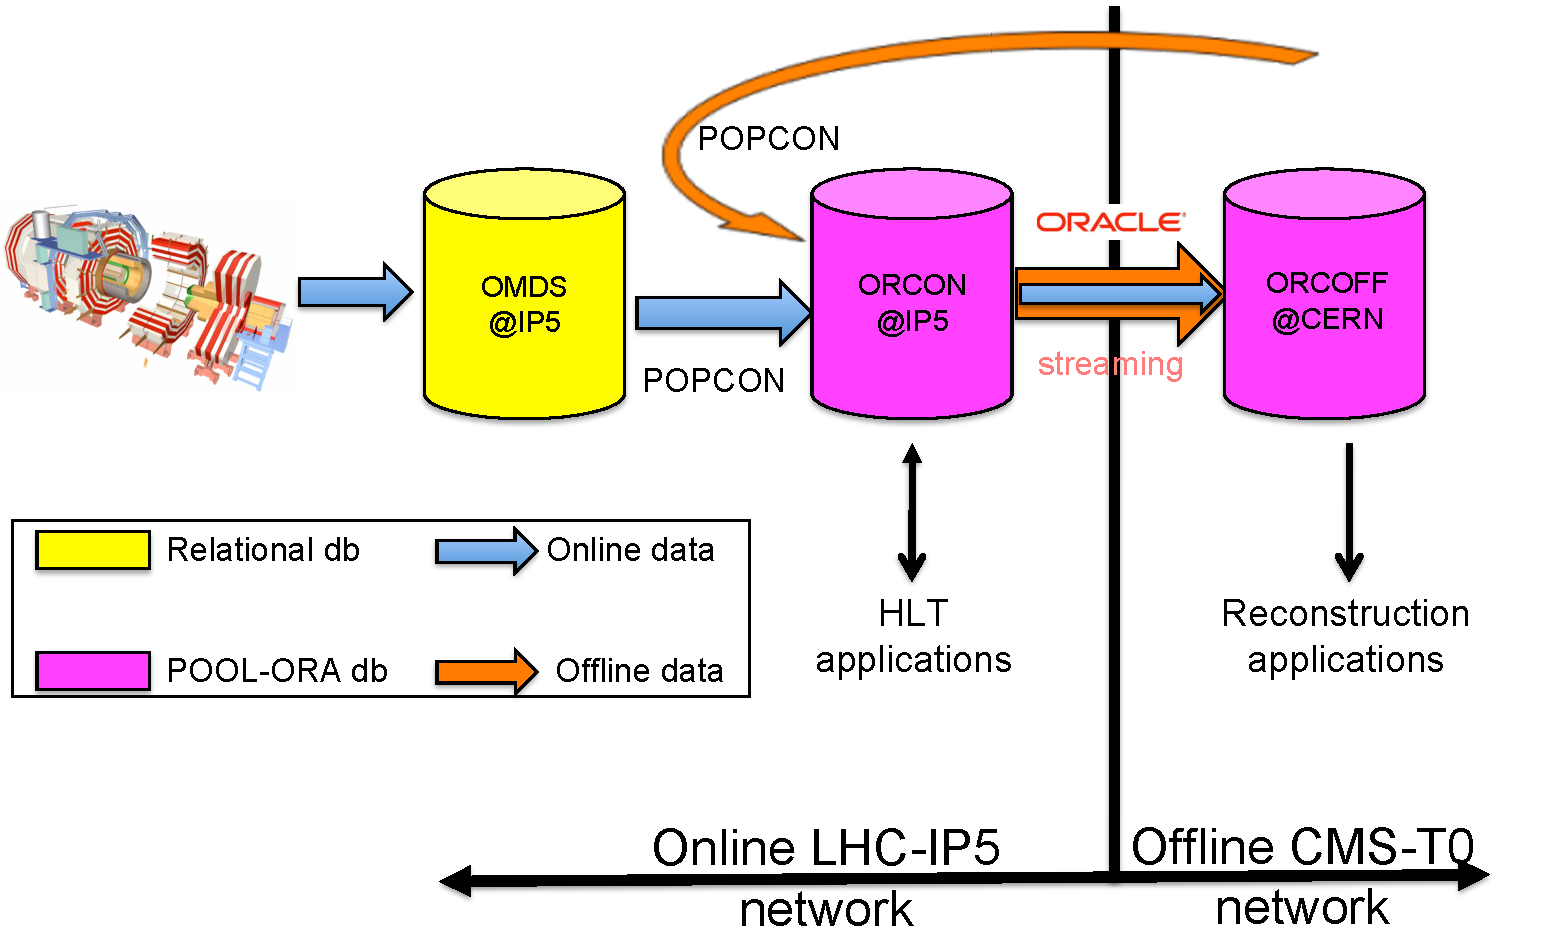
\includegraphics{figure/DBArchitecture.pdf}} \caption{Condition databases architecture.}
    \label{fig:CondDBArchitecture}
  \end{center}
\end{figure}
  
\section{Condition data description}
For each sub-detector the non-event data content of ORCON/ORCOFF can be classified in three main groups:
\begin {itemize}
\item {\bf Configuration data}: the data needed to bring the detector in running mode. 
This class includes voltage settings of power supplies, gas pressures, and any programmable parameter for front end electronics. 
\item {\bf Condition data}: the data from any detector subsystem describing its state, usually uploaded in OMDS directly from detector back-end devices. For example the Data Control System (DCS) information are stored with the ORACLE interface provided by PVSS. 
These data are mainly needed online for post mortem and detector error analysis. 
Only a subset of this data is transferred to the offline system (ORCON).  
\item {\bf Calibration data}: the data describing the calibration and alignment of the single pieces of the different sub-detectors. 
These quantities (such as pedestals offsets, drift values, noises, alignments, etc) are evaluated running offline dedicated algorithms. 
Since these data are needed both online, in order to be analyzed by the HLT algorithms, and offline, in order to reconstruct properly the physical quantities coming from collision events, they must be stored in the offline condition databases.
Therefore they should match the corresponding raw data coming from the collision events revealed by the detector.
\end{itemize}   
All these data need a tag and an interval of validity as meta-data. The interval of validity (IOV) is the contiguous (in time) set of events for which non-event data are to be used in reconstruction. 
According to the use-case, the IOV will be defined in terms of GPS-time (mainly for condition data) or ``run-number'' range (usually for calibrations). 
While the IOV for some electronic related conditions (e.g. pedestals and noises) is identical to the time interval in which these data were used in the online operations, some calibration data may posses an IOV different from the time range in which they have been defined.
For this reason, the IOV assignment for a given set of condition data is carried out at the offline level.
Each payload object, i.e. each data stored as POOL-ORA object in ORCOFF, is indexed by its IOV and a  tag, a label describing the calibration version, while the data themselves do not contain any time validity information.     

The matching with the raw data from the collision events is indeed possible via these meta-data: the reconstruction algorithms for the analysis of a given run query the offline condition data corresponding to the same run grouped through a set of tags, called \emph{global tag}.  


\section{Database architecture}\label{OffDB}
Different data usage and access from online to offline determines the overall architecture.
In the online network, the data are mainly written into the database, so that the time for a database transaction to be committed is critical, while, in the offline network, data are mainly read from the databases.
Moreover, the online data are being written at random time, while the offline data must be synchronized with the events.
Since online data are used for error tracking, different data items must be accessible in order to be compared between each other; on the other hand, offline data must be grouped before they are read, so that they can be decoded according to predefined rules.

The general data flow of non event data is described in figure \ref{fig:ConditionDataflow}: configuration data are prepared using the equipment management information and loaded into the detector (hardware and software). 
While running, the detector produces condition data, which are first stored in OMDS. 

The offline conditions subset is extracted and sent to the offline sites, as pictured in figure \ref{fig:CondDBArchitecture}. 
The condition data needed by the HLT farm will be loaded from ORCON. 
A software application named PopCon (Populator of Condition) operates the online to offline condition data transfer and encapsulates the relation data as POOL-ORA objects. 
 PopCon adds meta-data information (tag and IOV) to the condition data, so that they can be read by the offline/HLT software. 



Finally, data are transferred to ORCOFF, which is the main condition database for the CMS tier 0, using ORACLE streaming.

From ORCOFF data will be distributed to the other tier centers, through Frontier \cite{FRONTIER} packages. 
Calibration data will be written back to ORCON, using PopCon again, if required by the HLT. 
Collision event data are therefore processed using the offline condition data. 
As data taking goes on, we can understand better and better how the detector works; therefore, this will require new calibrations, hence new versions of condition data, identified by new tags.


\subsection{Online database}

The online database must allow for accessing individual, ideally self explaining data items: hence a pure ORACLE access and manipulation structure has been chosen for OMDS. 
Data size is expected to become very large (several TBs), and, since condition data will constantly flow into the DB, the time needed to store these data in OMDS is a critical issue. 

To fulfill these requirements, each sub-detector designed his own DB schema, reflecting as much as possible the detector structure.

 
\subsection{Offline database}

As shown in figure \ref{fig:CondDBArchitecture}, the CMS database infrastructure envisages two offline databases intended for condition data:
\begin{itemize} 
\item {\bf ORCON} is a part of the database infrastructure at P5, but is explicitly intended for offline purposes. 
It provides offline condition data for the HLT operation, and serves as a intermediate storage of the latest condition objects.      
\item {\bf ORCOFF} is the offline master database for condition data. 
It is located at T0 (at IT). 
It contains the entire history of all CMS condition data and serves as input source for both prompt reconstruction and condition deployment service at T1/T2 sides.
\end{itemize}

Both of them posses identical ``schemas'', optimized for the offline usage. 

Together with the production databases, CMS users can benefit also in using a ``development'' and an ``integration'' database intended for tests and accessible from the offline network: 
\begin{itemize}
\item{\bf INT2R}, offline database for preparation and development purposes. 
\item{\bf INT9R}, offline database for integration. It should be used when all the tests on INT2R have been succeded. 
\end{itemize}


The data access (both insertion and retrieval) is controlled only by the C++ based POOL-ORA API (see \ref{subsect:POOL-ORA}). The actual policy of the CMS community is to write any condition/calibration data in ORCON. The data are then copied to ORCOFF using the ORACLE streaming tool.
In section \ref{subsect:POPCON} more information about the online-to-offline (O2O) transfer operated by PopCon is given.    

\subsection{POOL Object Relational Database Access: POOL-ORA}\label{subsect:POOL-ORA}
POOL\cite{POOL}, the persistency framework for object storage for the LHC experiments, was successfully used by ATLAS, CMS and LHCb to handle data during data challenges. 
The relational back-end of POOL (POOL-ORA) is chosen by the CMS experiment for condition data handling. 
The implementation sits on top of a generic relational database layer. The POOL-ORA interface used for handling non-event data is identical to that of POOL-ROOT used  for handling event data. 
The main feature is that the transient object model drives the database model: the designers of the offline data model don't need to know the tabular representation of the data in the database. The offline database schema is automatically created from the definitions of the persistent-capable objects by following the Object Relational Mapping (ORM) rules. 
The data are retrieved from the underlying relational database, then materialized as \texttt{C++} objects in memory by following the dictionary information, hence finding the corresponding entries in the ORM mapping files.

As shown in figure \ref{fig:POOLORA}, PoolORA consists of three domains:
\begin{itemize}
\item {\bf COmmon Relational Access Layer (CORAL)} defines a vendor independent API for relational database access, data and schema manipulation. 
Three technology plugins, for ORACLE, MySQL and SQLite technologies, are released together with the API. 
\item {\bf Object Relational Access (ORA)} implements the object relational mapping mechanism and is responsible for transforming \texttt{C++} object definitions into relational structures and vice-versa.
\item {\bf Relational Storage Service} implements the POOL Storage Service using the relational Access and the Object Relational Access components. 
\end{itemize} 

 \begin{figure}[hbtp]
  \begin{center}
    \resizebox{0.7\textwidth}{!}{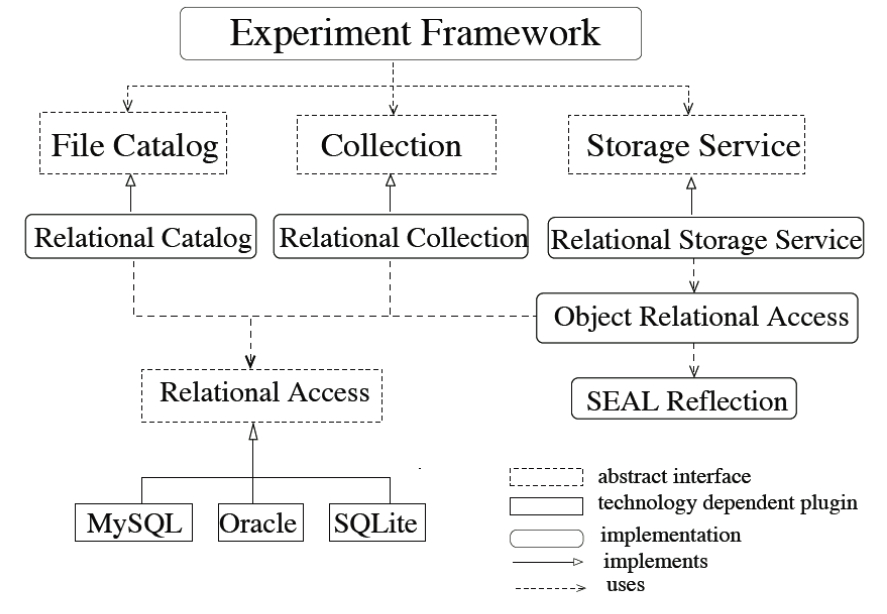
\includegraphics{figure/POOLOra.jpg}} \caption{POOL-ORA in the overall architecture.}
    \label{fig:POOLORA}
  \end{center}
\end{figure}
 
CMS contributes to the development of the POOL-ORA infrastructure in order to ensure that it satisfies the requirements from the CMS community.    


\subsection{PopCon}\label{subsect:POPCON}

PopCon \cite{PopCon} is a CMSSW\cite{CMSSW} mini-framework that transfer the conditions objects from a user-defined data source to ORCON.

Popcon is based on the \texttt{cmsRun} infrastructure, so the base PopCon application class is the EDAnalyzer. 
However, it is possible to use different data sources such as databases, ROOT files, ASCII files, etc. 
For each conditions object (payload) class a PopCon application is created.

The core framework consists of three parametrized classes, as can be seen in figure \ref{fig:PopConSchema}:

\begin{itemize}
\item PopCon
\item PopConSourceHandler
\item PopConAnalyzer 
\end{itemize}

The ``detector user'' provides the code which handles the data source and specifies the destination for the data, writing a derived class of PopConSourceHandler, where all the online (source handling) code goes. 
The user instantiates the objects, provides the IOV information for such objects and configures the database output module. 
PopCon configuration file associates the tag name defined according to some specific rules, to the condition object. 
Once the object is built, the PopCon application writes the data to the specified database. 
Subdetector code does not access the target output database: it only passes the objects to the output module.

The analyzer object holds the source handling object. It also serves some additional functionality such as:
\begin{itemize}
 \item Locking mechanism.
 \item Transfer logging.
 \item Payload verification (IOV sequence).
 \item Application state management.
 \item Database output service.
\end{itemize}
The writer in PopCon iterates over the container of user objects and stores it in the user-configured data destination. 

\begin{figure}[hbtp]
  \begin{center}
    \resizebox{1.0\textwidth}{!}{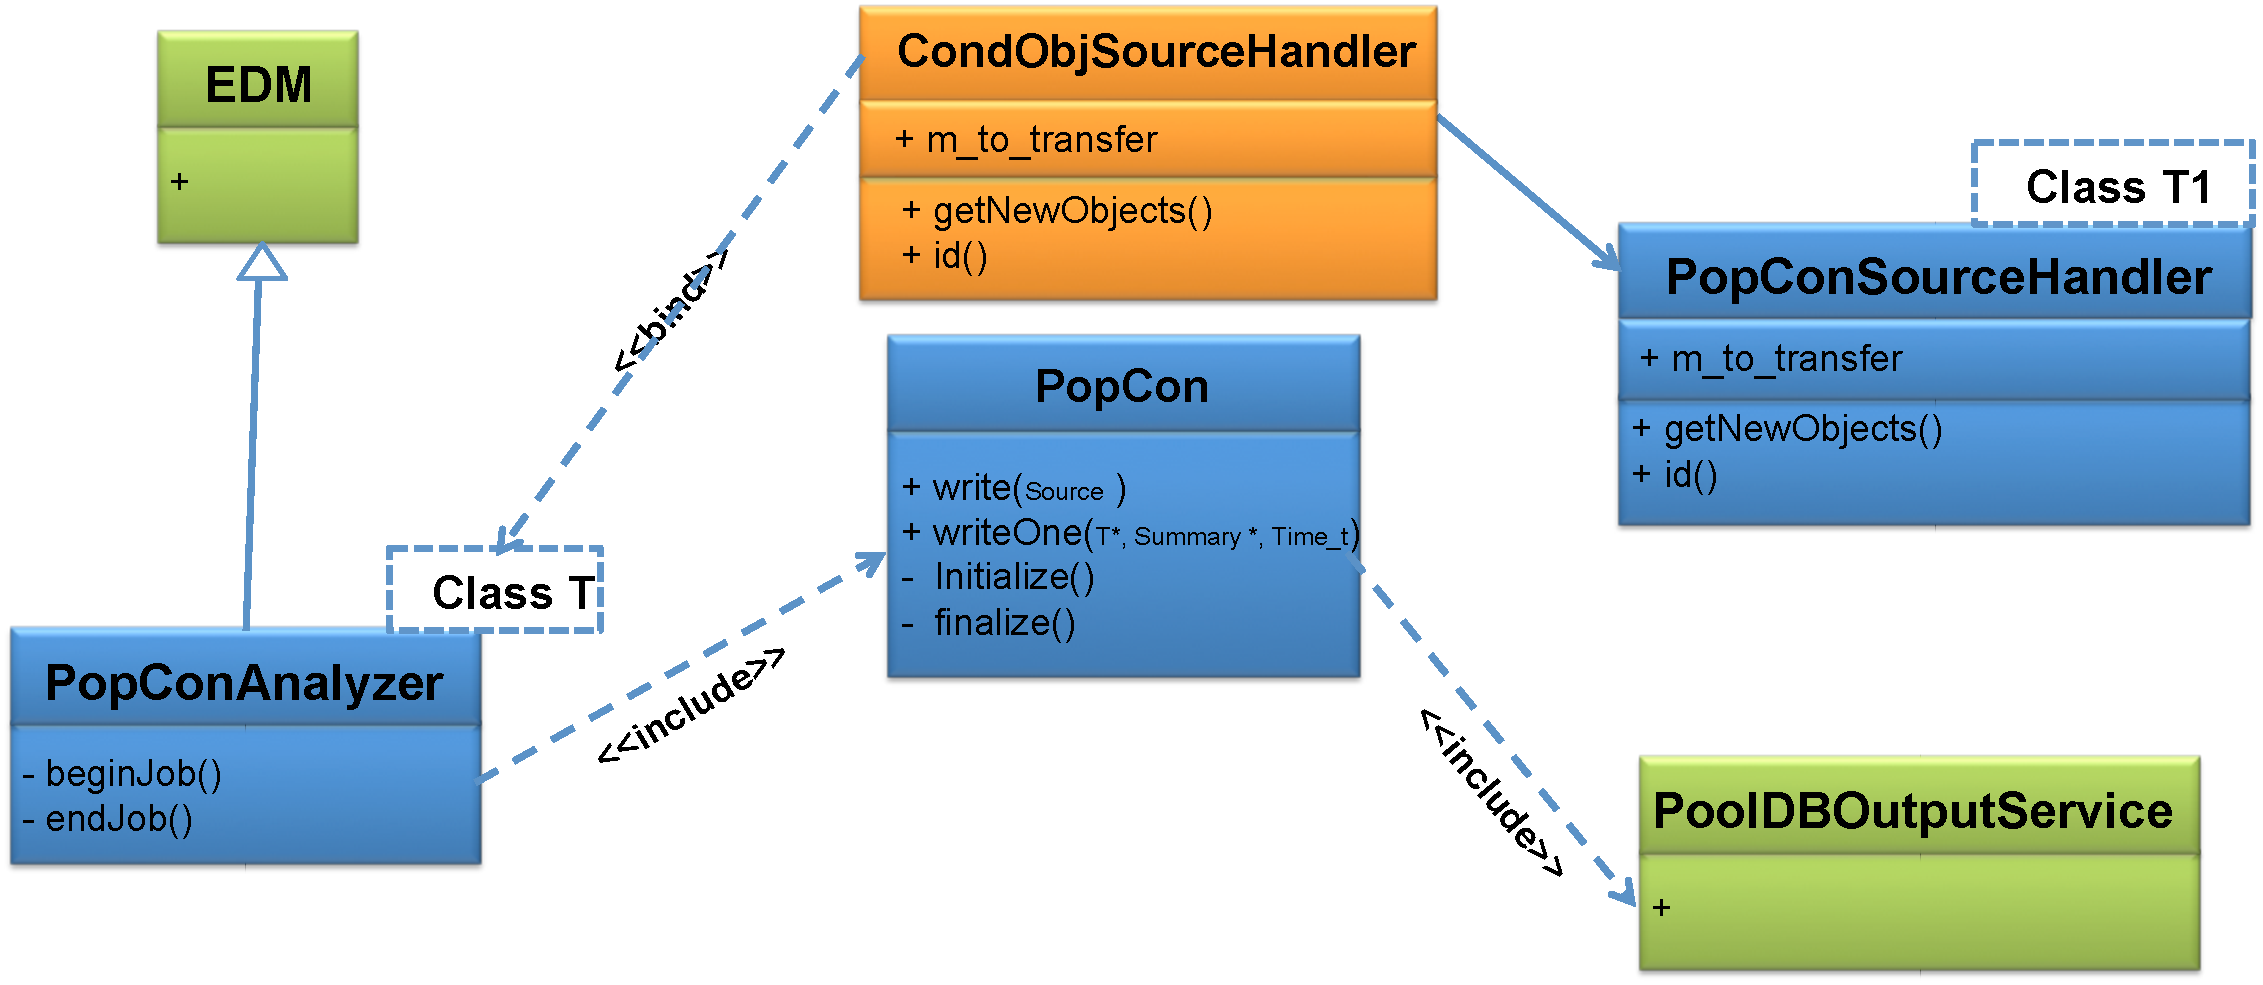
\includegraphics{figure/uml_popcon.pdf}}\caption{Schema of the classes for the PopCon package.}
    \label{fig:PopConSchema}
  \end{center}
\end{figure}

Any transaction towards ORCON is logged by PopCon, and the process information is sent to a database account as well. A monitoring tool for this information was developed, in order to check the correctness of the various transactions, and to keep trace of every upload for condition data.
 


\section{First experience in operating the population on the condition db in 2008 and 2009 }

In the 2008 and 2009 global runs (with and without the magnetic field) the great majority of the condition data was transferred offline with a PopCon application. 
Great effort was devoted by the CMS database project team in the integration of all the software and the infrastructural chain to upload the calibration constants into the CMS condition databases. 
Many tools were provided to help the sub-detector responsible people to populate the database. 
A central procedure, based on an automatic uploader into ORCON on a dedicated machine in the online network, was successfully deployed during 2008, and is the recommended way to populate ORCON in 2009 data taking. 


\subsection{Condition objects written with PopCon in 2008}

As stated, each condition data (pedestals, Lorentz Angles, drift time, etc.) corresponds to a {\texttt C++} object (``CondObjects'') into the CMS overall software. 
Each object is associated with a PopCon application which writes the payload into ORCON. 
Table \ref{tab:page_layout} lists all the CondObjects written by the corresponding sub-detector condition/calibration experts in 2008, grouped according to the subsystem they belong to. 
For each object the type, the approximate data size in ORCON and the uploading frequency are also reported.  
   
 \begin{table}[htbp]
    \caption{2008 CMS condition objects list}
    \label{tab:page_layout}
    \begin{center}
      \begin{tabular}{||c|c|c|c|c||} \hline 
            Subsystem   & Name & Type & Data size & Frequency\\  \hline
  \multirow{3}{*} {Pixel} & SiPixelFedCablingMap & online configuration& 1K& once (before the run )\\        
 & SiPixelLorentzAngle & offline calibration & 1MB & each run (if different) \\ 
 & SiPixelCalibConfiguration  & online calibrations & 5KB & each calibration run \\ \hline
  \multirow{5}{*} {Tracker} & SiStripFedCapling & online configuration& 1K&once \\        
& SiStripBadStrip & online condition & 1MB&  each run (if different)\\ 
& SiStripTreshold & offline calibration & 1MB&  each run (if different)\\        & SiStripPedestals & offline calibration & 1MB&  each run (if different)\\  
& SiStripNoise & offline calibration & 1MB&  each run (if different)            
\\ \hline

  \multirow{2}{*} {Ecal} & EcalPedestals & online calibration& 2MB& daily \\     & EcalLaserAPDPNRatios & online calibration & 2MB& hourly        
\\ \hline

 \multirow{5}{*} {Hcal} & HcalElectronicsMap & online configurations & 1MB& once (before the run)  \\  
& HcalGains & offline calibrations & 1MB& each run \\  
& HcalPedestals & offline calibrations & 1MB& each run \\  
& HcalPedestalsWidths & offline calibrations & 1MB& each run \\  
& HcalQIEData & online calibrations & 1MB& each run 

\\ \hline

 \multirow{7}{*} {CSC} & CSCChamberMap & online configuration & 10KB & monthly  \\  
& CSCCrateMap & online configuration & 10KB & monthly  \\  
& CSCDDUMap & online configuration & 10KB & monthly  \\  
& CSCChamberIndex & online configuration & 10KB & monthly  \\  
& CSCGains & offline calibrations & 2MB& each run  \\  
& CSCNoiseMatrix & offline calibrations & 2MB& each run  \\  
& CSCPedestals & offline calibrations & 2MB& each run  \\  
\hline

\multirow{5}{*} {DT} & DtReadOut & online configuration & 10MB & once  \\  
 & DtCCBConfig &  online configuration  & 100KB & once (before the run)   \\
 & DtT0 & offline calibration & 10MB & rare  \\
 & DtTTrig & offline calibration & 1MB & at trigger change   \\
 & DtMTime & offline calibration & 1MB & daily   \\
\hline


\multirow{3}{*} {RPC} & RPCEMap & online configuration & 10MB & once  \\
& L1RPCConfig & online configuration & 10MB & once  \\
& RPCCond & online conditions & 10MB & daily  \\
\hline

\multirow{1}{*} {DAQ} & RunSummary & run conditions & 10KB & run start/end  \\
\hline
      \end{tabular}
    \end{center}
  \end{table}


\subsection{Central population of the condition database}

A central procedure was set up in 2008, and used since then, for populating the CMS condition databases: it exploits a central account, explicitly devoted to condition database population, in the CMS online network. 
On that account a set of automatic jobs were centrally set up for any single sub-detector user, in order to both populate ORCON and monitor any transaction to it. 

Two possibilities are given to users:
\begin{enumerate}
\item to run automatically the application that reads from any online source, assigns tag and interval of validity, and uploads the constants into ORCON (mainly for condition). 
The time interval of the automatic jobs are negotiated with the users;  
\item to use the account as a drop-box: users copy the calibrations in the SQLite\cite{SQLite} format into a dedicated folder for each sub-detector, and then these data are automatically exported in ORCON (mainly for offline calibrations).  
\end{enumerate}

Figure \ref{fig:DropBox} shows a sketch of the central system to populate the condition database. Each sub-detector responsible person may transfer the payload on the central machine, that runs automatically the exportation into ORCON (referred as  ``SubdetectorExport'' scripts). Other automatic scripts (referred as ``SubdetectorO2O'' scripts in the figure), indeed, control that new conditions have appeared in the online table, and, if that is the case, perform the data transfer from OMDS to ORCOFF.   

The PopCon applications run transfer each payload into the corresponding account, and all the log information in the PopConLog account on ORCON itself. 
    




\begin{figure}[hbtp]
  \begin{center}
    \resizebox{1.0\textwidth}{!}{\includegraphics{figure/PopConCentral}} \caption{Schematic illustration of the central system to populate ORCON, and of the web monitoring system.}
    \label{fig:DropBox}
  \end{center}
\end{figure}

Each automatic job is associated with a ``watchdog'' tool that monitors its status.
The job monitoring information are also logged into the PopConLog account on ORCON.  

A dedicated web monitor, {\it PopCon monitoring} \cite{PopConMonitoring}  was set up on a CMS web server in order to look at all the logged information, hence monitoring the activity on the condition databases. 


\emph{PopCon monitoring} is structured in five main components (see figure \ref{fig:PopConGuiArchitecture}):

\begin{figure}[htbp]
\begin{center}
\resizebox{0.8\textwidth}{!}{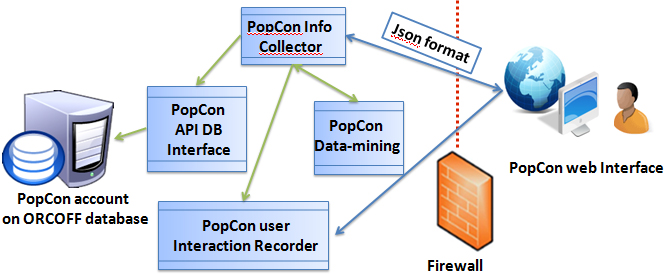
\includegraphics{figure/popConGuiArchit.jpg}}
\end{center}
\caption{PopCon monitoring Architecture} \label{fig:PopConGuiArchitecture}
\end{figure}


\begin{itemize}
\item the \textbf{PopCon API DB Interface} retrieves the
entities monitored by PopCon;
\item the \textbf{PopCon user Interaction Recorder} is a collection 
that retains an interaction history by each user.
\item the \textbf{PopCon data-mining} extracts patterns from data, 
entities monitored by PopCon. 
and the history of recorded user interactions, 
hence transforming them into information such as warnings, errors or alarms according to use case models.
\item  the \textbf{PopCon info collector} aggregates the
information produced by the different database transactions 
and the history of recorded user interactions, and encodes them in JSON\footnote{JSON (JavaScript Object Notation) is a lightweight data-interchange format.} format.
\item the \textbf{PopCon Web Interface} displays the information about the database transactions 
from the different user perspectives,
organizing data in tables (see figure \ref{fig:popConTable}) and/or charts (see figure \ref{fig:PopConAct}).
\end{itemize}


\begin{figure}[htbp]
\resizebox{1.0\textwidth}{!}{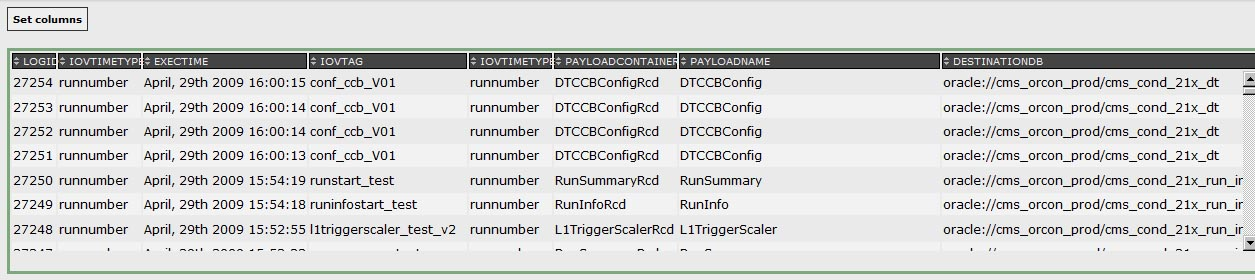
\includegraphics{figure/popConTable.jpg}}
\caption{\label{fig:popConTable} 
The PopCon web interface represents information about database transactions in 
different types: both charts and tables.
A user can easily add or remove columns by clicking the checkbox
and also columns can be sorted. Information could be grouped according to different filters.
%As table is possible to click on a column header and the columns are sorted.
%To add or delate columns, click set columns. 
}
\end{figure}
Finally two important monitor web pages are produced:
\begin{enumerate}
\item an activity summary, in which the number of transactions towards ORCON, the subsystem involved, the IOV and tag uploaded can be displayed, according to the users' requests. An example is shown in figure \ref{fig:PopConAct}. 
\item the logs of all the central scripts, as produced by the watchdog tools. Looking at those logs, the correct behaviour of the central uploader machine is controlled, so that an alarm system, based on that information, can recognize if some exportations were not successful and, eventually, inform the end-user of the error occurred. A screenshot of the page is in figure~\ref{fig:WatchDog}.    
\end{enumerate}


\begin{figure}[hbtp]
  \begin{center}
    \resizebox{1.0\textwidth}{!}{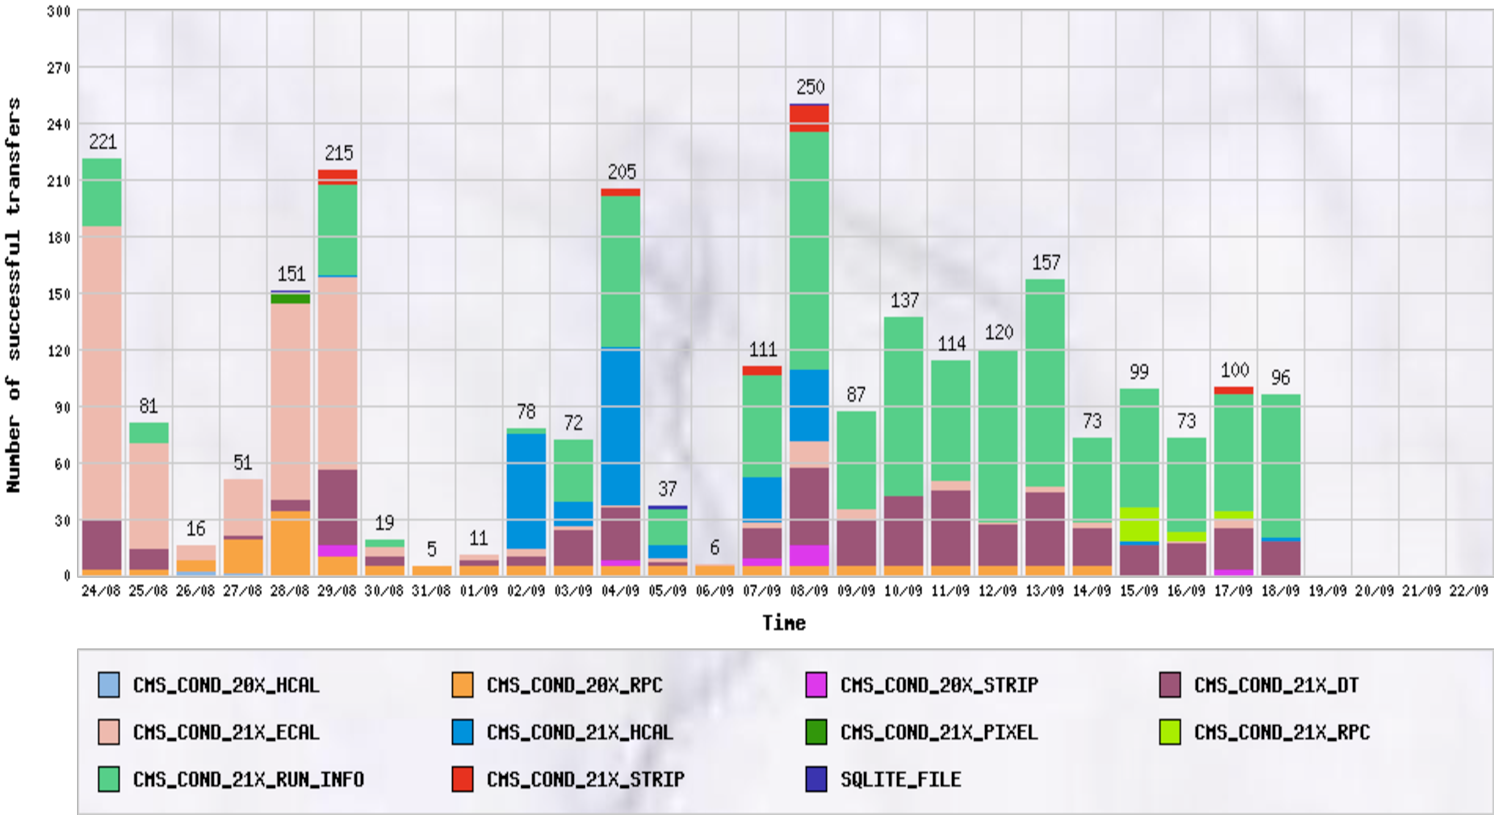
\includegraphics{figure/PopConAct.pdf}} \caption{PopCon activity during end September-beginning of October 2008.}
    \label{fig:PopConAct}
  \end{center}
\end{figure}


\begin{figure}[hbtp]
\resizebox{1.0\textwidth}{!}{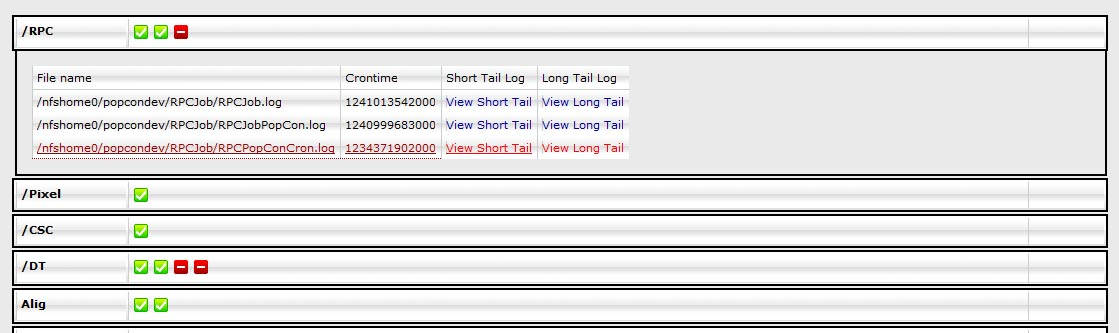
\includegraphics{figure/errorGUI.jpg}} \caption{Screenshot of the web page produced by the monitoring system that checks the watchdog tools for the automatic population of ORCON. Different colours helps to identify, quickly, the seriousness of the problem.}
  \label{fig:WatchDog}
\end{figure}

Figure \ref{fig:PopConAct} reports all the transactions towards the condition database accounts occurred in a month of cosmic data taking in 2008. 
As the summary plot points out, almost all sub-detectors did use PopCon to upload calibration constants to the condition databases.
An average of one hundred PopCon applications per day were run during the test runs in summer/fall 2008, hence one hundred connections per day to the condition databases took place.


During the entire year 2008 the total amount of condition data written in the production database was approximatively 1 TB. 
Indeed, no network problems, neither for the online-offline streaming, nor for Frontier were detected. 
All the conditions and calibrations were properly evaluated for CRUZET and CRAFT data taken in 2008, and are being evaluated in currunt 2009 CRAFT runs, leading to several global tags used for the reconstruction and the analysis of the cosmic ray data by the whole CMS community. 


\section{Conclusion}

A database system was set up in order to upload, store and retrieve all calibration constants for the CMS experiment. 
The system relies on ORACLE database for data storage, and on the PoolORA technology for the HLT and offline data. PopCon CMSSW application operates the population of ORCON and add some additional services such as the transaction logging, hence the monitoring.  
The whole chain was deployed and tested succesfully during 2008 challenges with cosmic rays: these tests pointed out that the system we have just described is stable and robust enough for the 2009-2010 collision data taking.

\begin{thebibliography}{9}
 \bibitem {POOLORA} POOL PERSISTENCY FRAMEWORK FOR THE LHC NEW DEVELOPMENTS AND CMS APPLICATIONS, Z.Xie et al. { \em  Proc. ``Frontier Science 2005: New Frontiers in Sub nuclear Physics, September 12-17,2005 Milan, Italy''}
  
 \bibitem{PVSS} The Joint COntrols Project Framework, M. Gonzalez-Berges {\em Int. Conf. on Computing in High Energy Physics, March 2003, La Jolla, California}.

\bibitem{FRONTIER} CMS conditions data access using FroNTier, B.Blumenfeld et al. {\em 2008 J. Phys.: Conf. Ser. 119 072007}.
\bibitem{POOL}  THE LCG POOL Project - General Overview and Project Structure, D.Dullman et al., { \em Proc. CHEP 2003 MOKToo7, La Jolla, March 24-28 2003}
 \bibitem{CMSSW} Analysis environments for CMS, C.D. Jones et al. {\em J. Phys.: Conf. 2008 Ser. 119 032027 }
\bibitem {PopCon} First experience in operating the population of the condition database of the CMS experiment, M.De Gruttola et al. {\em Computing in High-Energy Physics Conference (CHEP '09), Prague, Czech Repiblic, 23 March - 27 March 2009, Distributed Processing and Analysis track}.
\bibitem{SQLite} http://www.sqlite.org/
\bibitem{PopConMonitoring}  PopCon monitoring: web application for detailed real-time database transaction monitoring, Ignas Butenas et al. {\em The 15th International Conference on Distributed Multimedia Systems, San Francisco Bay, USA
September 10 - September 12, 2009.} 



\end{thebibliography}

\end{document}










%==============================================================================
% title page for many authors
%
%\begin{titlepage}
%  \internalnote{2005/000}
%  \title{CMS Technical Note Template}
%
%  \begin{Authlist}
%    A.~Author\Iref{cern}, B.~Author\Iref{cern}, C.~Author\IAref{cern}{a},
%    D.~Author\IIref{cern}{ieph}, E.~Author\IIAref{cern}{ieph}{b},
%    F.~Author\Iref{ieph}
%  \end{Authlist}
%
%  \Instfoot{cern}{CERN, Geneva, Switzerland}
%  \Instfoot{ieph}{Institute of Experimental Physics, Hepcity, Wonderland}
%  \Anotfoot{a}{On leave from prison}
%  \Anotfoot{b}{Now at the Moon}
%
%  \begin{abstract}
%    This is a template of a CMS paper, written in LaTeX,
%    processed with {\it cmspaper.sty} style.
%    It is based on the {\it cernart.sty} and {\it articlet.sty} styles.
%    There are two versions of the title page.
%    The current one is designed for many authors.
%    The one on the previous page is for few authors.
%    Just delete the one which you do not need.
%  \end{abstract} 
%  
%\end{titlepage}
%
%==============================================================================

\section{CMS papers}

    There are three kind of CMS papers: ``CMS Note'', 
    ``CMS Internal Note'' and ``CMS Conference Report''.
    They differ only in the header of the first page,
    which includes an eps figure different for each kind.
    One of the following commands must be selected,
    where \verb$yyyy$ is the current year
    and \verb$xxx$ is the document number allocated by the CMS secretariat:
{\small \begin{verbatim}
  \cmsnote{yyyy-xxx}
  \internalnote{yyyy-xxx}
  \conferencereport{yyyy-xxx}
\end{verbatim} }
    
Apart from the title and authors some supplementary information can be given
on the first page:
{\small \begin{verbatim}
  \collaboration{Physics Analysis Group}
  \conference{Presented at {\em Hard Collisions}, Coconut Island, May 2005}
  \submitted{Submitted to {\em Physics Rumours}}
  \note{Preliminary version}
\end{verbatim} }

\subsection{Subsection}

This is an example of subsection

\subsubsection{Subsubsection}

This is an example of subsubsection

\section{Document layout}

\subsection{Page size, margins and fonts}

Use only very standard PostScript fonts: 
%    \begin{center}
      \begin{tabular}{|l|ccc|} \hline
         LaTeX name & roman & sansserif & typewriter \\
         PostScript name & Times & Helvetica & Courrier \\ \hline
      \end{tabular}
%    \end{center}

  European A4 paper size is 210 mm x 297 mm (8.3" x 11.7").
  American paper is 6 mm (0.2") wider and 18 mm (0.7") shorter, 
  thus it has 216 mm x 279 mm (8.5" x 11.0").
  In this template we have set the LATEX page style parameters as follows:
{\small \begin{verbatim}
  \hoffset and \voffset are reset to 0
  \oddsidemargin, \evensidemargin and \marginparwidth = 25mm
  \marginparsep is set equal to \baselineskip
  \topmargin=20mm, \headheight=0, \headsep=0
  \footskip=6mm
  \textwidth=16cm
  \textheight is set to NN\baselineskip, where NN is 57, 51 or 46 ....
\end{verbatim} }

  These settings lead to margins, measured from the edge of the physical page, 
  as listed in Tab.~\ref{tab:page_layout}.
  In this table "foot" is the space left below the page number (footer).

  The paper size used in generating the PostScript file is defined by 
  the {\em -t papertype} option in {\em dvips} 
  where {\em papertype} stands for {\em a4} or {\em letter}.

  \begin{table}[htb]
    \caption{Page layout for A4 and US letter formats.}
    \label{tab:page_layout}
    \begin{center}
      \begin{tabular}{|l|ccccc|ccccc|} \hline
               & \multicolumn{5}{c|}{mm} & \multicolumn{5}{c|}{inches} \\ 
        margin & left & right & top & bottom & foot &
                 left & right & top & bottom & foot \\ \hline
        A4 & 25 & 25 & 20 & 34 & 28 & 1.0 & 1.0 & 0.8 & 1.3 & 0.9 \\
        US letter   & 25 & 31 & 20 & 16 & 10 & 1.0 & 1.2 & 0.8 & 0.6 & 0.4 \\ \hline
      \end{tabular}
    \end{center}
  \end{table}

\subsection{Tables, figures}

Small tables can be inside the text in a fixed place, as the table with
the font names above. Bigger tables should be defined as floating bodies
and have a caption and label as Tab.~\ref{tab:page_layout} above.

Figures can be inserted as EPS files using package {\em graphics},
automaticaly called by {\em cmspaper.cls}.
Specifying both width and height forces both dimensions to be changed.
If one of the dimensions is omitted the aspect ratio is preserved.
If no one is given, the size is taken from the {\em \%\%BoundingBox}
(see examples in Fig.~\ref{fig:ex1} and \ref{fig:ex2}).

\begin{figure}[hbtp]
  \begin{center}
    \resizebox{3cm}{!}{\includegraphics{cmslogo}}
    \caption{Figure inserted by 
      \tt $\backslash$resizebox\{3cm\}\{!\}\{$\backslash$includegraphics\{cmslogo.eps\}\}.}
    \label{fig:ex1}
  \end{center}
\end{figure}

\begin{figure}[hbtp]
  \begin{center}
    \resizebox{5cm}{1cm}{\includegraphics{cmslogo}}
    \caption{Figure inserted by 
       \tt $\backslash$resizebox\{5cm\}\{1cm\}\{$\backslash$includegraphics\{cmslogo.eps\}\}.}
    \label{fig:ex2}
  \end{center}
\end{figure}

Quite often it is convenient to place 2 figures side by side as a single
floating body. An environment {\em 2figures} is provided for that
(see Fig.~\ref{fig:ex3} and \ref{fig:ex4}).

\begin{2figures}{hbtp}
  \resizebox{\linewidth}{0.5\linewidth}{\includegraphics{cmslogo}} &
  \resizebox{\linewidth}{0.5\linewidth}{\includegraphics{cmslogo}} \\
%  \resizebox{\linewidth}{!}{\includegraphics{cmslogo.eps}} &
%  \resizebox{\linewidth}{!}{\includegraphics{cmslogo.eps}} \\
  \caption{The left figure}
  \label{fig:ex3} &
  \caption{The right figure}
  \label{fig:ex4} \\
\end{2figures}

%------------------------------------------------------------------------------

\section{Submitting a note}

Please follow the rules and procedures defined on the CMSDOC server, or request them by e-mail to:\begin{center} {\em cmsnotes@cmsdoc.cern.ch} \end{center}

\section{Reference example}

References should be placed at the end of the note 
(see example \cite{NOTE000}).

\begin{thebibliography}{9}
  \bibitem {NOTE000} {\bf CMS Note 2005/000},
    X.Somebody et al.,
    {\em "CMS Note Template"}.
\end{thebibliography}
 
%------------------------------------------------------------------------------
\pagebreak

{\small \begin{flushleft}
Appendix: A4/US page set-up\\
-1 - - - - - - - - - - - - - - - - - - - - - - - - - - - - - - - - - - - - - -\\
-2 - - - - - - - - - - - - - - - - - - - - - - - - - - - - - - - - - - - - - -\\
-3	
	See section 2.1\\
-4 - - - - - - - - - - - - - - - - - - - - - - - - - - - - - - - - - - - - - -\\
-5 - - - - - - - - - - - - - - - - - - - - - - - - - - - - - - - - - - - - - -\\
-6 - - - - - - - - - - - - - - - - - - - - - - - - - - - - - - - - - - - - - -\\
-7 - - - - - - - - - - - - - - - - - - - - - - - - - - - - - - - - - - - - - -\\
-8 - - - - - - - - - - - - - - - - - - - - - - - - - - - - - - - - - - - - - -\\
-9 - - - - - - - - - - - - - - - - - - - - - - - - - - - - - - - - - - - - - -\\
10 - - - - - - - - - - - - - - - - - - - - - - - - - - - - - - - - - - - - - -\\
-1 - - - - - - - - - - - - - - - - - - - - - - - - - - - - - - - - - - - - - -\\
-2 - - - - - - - - - - - - - - - - - - - - - - - - - - - - - - - - - - - - - -\\

-3 - - - - - - - - - - - - - - - - - - - - - - - - - - - - - - - - - - - - - -\\
-4 - - - - - - - - - - - - - - - - - - - - - - - - - - - - - - - - - - - - - -\\
-5 - - - - - - - - - - - - - - - - - - - - - - - - - - - - - - - - - - - - - -\\
-6 - - - - - - - - - - - - - - - - - - - - - - - - - - - - - - - - - - - - - -\\
-7 - - - - - - - - - - - - - - - - - - - - - - - - - - - - - - - - - - - - - -\\
-8 - - - - - - - - - - - - - - - - - - - - - - - - - - - - - - - - - - - - - -\\
-9 - - - - - - - - - - - - - - - - - - - - - - - - - - - - - - - - - - - - - -\\
20 - - - - - - - - - - - - - - - - - - - - - - - - - - - - - - - - - - - - - -\\
-1 - - - - - - - - - - - - - - - - - - - - - - - - - - - - - - - - - - - - - -\\
-2 - - - - - - - - - - - - - - - - - - - - - - - - - - - - - - - - - - - - - -\\
-3 - - - - - - - - - - - - - - - - - - - - - - - - - - - - - - - - - - - - - -\\
-4 - - - - - - - - - - - - - - - - - - - - - - - - - - - - - - - - - - - - - -\\
-5 - - - - - - - - - - - - - - - - - - - - - - - - - - - - - - - - - - - - - -\\
-6 - - - - - - - - - - - - - - - - - - - - - - - - - - - - - - - - - - - - - -\\
-7 - - - - - - - - - - - - - - - - - - - - - - - - - - - - - - - - - - - - - -\\
-8 - - - - - - - - - - - - - - - - - - - - - - - - - - - - - - - - - - - - - -\\
-9 - - - - - - - - - - - - - - - - - - - - - - - - - - - - - - - - - - - - - -\\
30 - - - - - - - - - - - - - - - - - - - - - - - - - - - - - - - - - - - - - -\\
-1 - - - - - - - - - - - - - - - - - - - - - - - - - - - - - - - - - - - - - -\\
-2 - - - - - - - - - - - - - - - - - - - - - - - - - - - - - - - - - - - - - -\\
-3 - - - - - - - - - - - - - - - - - - - - - - - - - - - - - - - - - - - - - -\\
-4 - - - - - - - - - - - - - - - - - - - - - - - - - - - - - - - - - - - - - -\\
-5 - - - - - - - - - - - - - - - - - - - - - - - - - - - - - - - - - - - - - -\\
  -6 - - - - - - - - - - - - - - - - - - - - - - - - - - - - - - - - - - - - - -\\
-7 - - - - - - - - - - - - - - - - - - - - - - - - - - - - - - - - - - - - - -\\
-8 - - - - - - - - - - - - - - - - - - - - - - - - - - - - - - - - - - - - - -\\
-9 - - - - - - - - - - - - - - - - - - - - - - - - - - - - - - - - - - - - - -\\
40 - - - - - - - - - - - - - - - - - - - - - - - - - - - - - - - - - - - - - -\\
-1 - - - - - - - - - - - - - - - - - - - - - - - - - - - - - - - - - - - - - -\\
-2 - - - - - - - - - - - - - - - - - - - - - - - - - - - - - - - - - - - - - -\\
-3 - - - - - - - - - - - - - - - - - - - - - - - - - - - - - - - - - - - - - -\\
-4 - - - - - - - - - - - - - - - - - - - - - - - - - - - - - - - - - - - - - -\\
-5 - - - - - - - - - - - - - - - - - - - - - - - - - - - - - - - - - - - - - -\\
-6 - - - - - - - - - - - - - - - - - - - - - - - - - - - - - - - - - - - - - -\\
-7 - - - - - - - - - - - - - - - - - - - - - - - - - - - - - - - - - - - - - -\\
-8 - - - - - - - - - - - - - - - - - - - - - - - - - - - - - - - - - - - - - -\\
-9 - - - - - - - - - - - - - - - - - - - - - - - - - - - - - - - - - - - - - -\\
50 - - - - - - - - - - - - - - - - - - - - - - - - - - - - - - - - - - - - - -\\
-1 - - - - - - - - - - - - - - - - - - - - - - - - - - - - - - - - - - - - - -\\
-2 - - - - - - - - - - - - - - - - - - - - - - - - - - - - - - - - - - - - - -\\
-3 - - - - - - - - - - - - - - - - - - - - - - - - - - - - - - - - - - - - - -\\
-4 - - - - - - - - - - - - - - - - - - - - - - - - - - - - - - - - - - - - - -\\
-5 - - - - - - - - - - - - - - - - - - - - - - - - - - - - - - - - - - - - - -\\
-6 - - - - - - - - - - - - - - - - - - - - - - - - - - - - - - - - - - - - - -\\
-7 - - - - - - - - - - - - - - - - - - - - - - - - - - - - - - - - - - - - - -\\
-8 - - - - - - - - - - - - - - - - - - - - - - - - - - - - - - - - - - - - - -\\
-9 - - - - - - - - - - - - - - - - - - - - - - - - - - - - - - - - - - - - - -\\
60 - - - - - - - - - - - - - - - - - - - - - - - - - - - - - - - - - - - - - -\\
-1 - - - - - - - - - - - - - - - - - - - - - - - - - - - - - - - - - - - - - -\\
-2 - - - - - - - - - - - - - - - - - - - - - - - - - - - - - - - - - - - - - -\\
-3 - - - - - - - - - - - - - - - - - - - - - - - - - - - - - - - - - - - - - -\\
-4 - - - - - - - - - - - - - - - - - - - - - - - - - - - - - - - - - - - - - -\\
-5 - - - - - - - - - - - - - - - - - - - - - - - - - - - - - - - - - - - - - -\\
-6 - - - - - - - - - - - - - - - - - - - - - - - - - - - - - - - - - - - - - -\\
-7 - - - - - - - - - - - - - - - - - - - - - - - - - - - - - - - - - - - - - -\\
-8 - - - - - - - - - - - - - - - - - - - - - - - - - - - - - - - - - - - - - -\\
-9 - - - - - - - - - - - - - - - - - - - - - - - - - - - - - - - - - - - - - -\\
70 - - - - - - - - - - - - - - - - - - - - - - - - - - - - - - - - - - - - - -\\
-1 - - - - - - - - - - - - - - - - - - - - - - - - - - - - - - - - - - - - - -\\
-2 - - - - - - - - - - - - - - - - - - - - - - - - - - - - - - - - - - - - - -\\
-3 - - - - - - - - - - - - - - - - - - - - - - - - - - - - - - - - - - - - - -\\
-4 - - - - - - - - - - - - - - - - - - - - - - - - - - - - - - - - - - - - - -\\
-5 - - - - - - - - - - - - - - - - - - - - - - - - - - - - - - - - - - - - - -\\
-6 - - - - - - - - - - - - - - - - - - - - - - - - - - - - - - - - - - - - - -\\
-7 - - - - - - - - - - - - - - - - - - - - - - - - - - - - - - - - - - - - - -\\
-8 - - - - - - - - - - - - - - - - - - - - - - - - - - - - - - - - - - - - - -\\
-9 - - - - - - - - - - - - - - - - - - - - - - - - - - - - - - - - - - - - - -\\
80 - - - - - - - - - - - - - - - - - - - - - - - - - - - - - - - - - - - - - -\\
-1 - - - - - - - - - - - - - - - - - - - - - - - - - - - - - - - - - - - - - -\\
-2 - - - - - - - - - - - - - - - - - - - - - - - - - - - - - - - - - - - - - -\\
-3 - - - - - - - - - - - - - - - - - - - - - - - - - - - - - - - - - - - - - -\\
-4 - - - - - - - - - - - - - - - - - - - - - - - - - - - - - - - - - - - - - -\\
-5 - - - - - - - - - - - - - - - - - - - - - - - - - - - - - - - - - - - - - -\\
-6 - - - - - - - - - - - - - - - - - - - - - - - - - - - - - - - - - - - - - -\\
-7 - - - - - - - - - - - - - - - - - - - - - - - - - - - - - - - - - - - - - -\\
-8 - - - - - - - - - - - - - - - - - - - - - - - - - - - - - - - - - - - - - -\\
-9 - - - - - - - - - - - - - - - - - - - - - - - - - - - - - - - - - - - - - -\\
90 - - - - - - - - - - - - - - - - - - - - - - - - - - - - - - - - - - - - - -\\
-1 - - - - - - - - - - - - - - - - - - - - - - - - - - - - - - - - - - - - - -\\
-2 - - - - - - - - - - - - - - - - - - - - - - - - - - - - - - - - - - - - - -\\
-3 - - - - - - - - - - - - - - - - - - - - - - - - - - - - - - - - - - - - - -\\
-4 - - - - - - - - - - - - - - - - - - - - - - - - - - - - - - - - - - - - - -\\
-5 - - - - - - - - - - - - - - - - - - - - - - - - - - - - - - - - - - - - - -\\
-6 - - - - - - - - - - - - - - - - - - - - - - - - - - - - - - - - - - - - - -\\
-7 - - - - - - - - - - - - - - - - - - - - - - - - - - - - - - - - - - - - - -\\
-8 - - - - - - - - - - - - - - - - - - - - - - - - - - - - - - - - - - - - - -\\
-9 - - - - - - - - - - - - - - - - - - - - - - - - - - - - - - - - - - - - - -\\
100- - - - - - - - - - - - - - - - - - - - - - - - - - - - - - - - - - - - - -\\
\end{flushleft} }


